	\section*{Exercice 4 (5 points)}
\subsection*{1. On note $f'$ la fonction dérivée de $f$.}
\subsubsection*{a. Montrer que, pour tout réel $x$, $f'(x) = 3\left(x + \dfrac{1}{3}\right)(x - 1)$.}
	
	La fonction polynôme $f$ est dérivable sur $\mathbb{R}$ et donc sur $[0; +\infty[$ :
\begin{align*}
	f'(x)& = 3x^2 - 2x - 1 \\
	&= 3(x^2 - \dfrac{2}{3}x) - 1 \\
	&= 3\left[\left(x - \dfrac{1}{3}\right)^2 - \dfrac{1}{9}\right] - 1\\
&= 3\left[\left(x - \dfrac{1}{3}\right)^2 - \dfrac{4}{9}\right]\\
& = 3\left(x + \dfrac{1}{3}\right)(x - 1)
\end{align*}
On pouvait aussi développer l'expression proposée dans l'énoncé et prouver qu'elle est bien égale à la dérivée obtenue sous forme développée.
	\subsubsection*{b. En déduire le tableau de variation de $f$ sur $[0; +\infty[$.}
	
	Comme pour $x > 0$, $3\left(x + \dfrac{1}{3}\right) > 0$, le signe de $f'(x)$ est celui de $x - 1$, donc :
	\begin{itemize}
		\item Si $0 \leq x < 1$, $f'(x) < 0$ : la fonction est décroissante sur $[0; 1[$ ;
		\item Si $x > 1$, $f'(x) > 0$ : la fonction est croissante sur $[1; +\infty[$ ;
		\item $f(1) = 1 - 1 - 1 - 1 = -2$ est le minimum de la fonction sur $[0; +\infty[$.
	\end{itemize}
	
	\begin{center}
			\begin{tikzpicture}[double distance=2pt]
			\tkzTabInit{$x$/1,$f'(x)$/1,$f(x)$/2}{$0$,$1$, $+\infty$}
			\tkzTabLine{,-,z, +}
			\tkzTabVar{+/,-/ $-2$ /, +/}
		\end{tikzpicture}
	\end{center}
	\subsubsection*{c. Déterminer l’abscisse du point de la courbe représentative de $f$ pour lequel le coefficient directeur de la tangente vaut 7.}
	
Il faut trouver le nombre réel $x$ de $[0; +\infty[$ tel que :
	\[
	f'(x) = 7 \iff 3x^2 - 2x - 1 = 7 \iff 3x^2 - 2x - 8 = 0
	\]
	
	\[
	\Delta = 4 + 4 \times 3 \times 8 = 4 + 96 = 100 = 10^2 > 0
	\]
Cette équation a deux solutions :
	\[
	x_1 = \dfrac{2 + 10}{6} = 2 \quad \text{et} \quad x_2 = \dfrac{2 - 10}{6} = -\dfrac{4}{3}
	\]
Seule la première solution est positive, donc $f'(2) = 7$.
	
	\subsection*{2. On note $x_0$ l’unique solution de l’équation $f(x) = 0$. On admet que $x_0 \in [1; 2]$.}
	
	\subsubsection*{a. On considère la fonction suivante définie en langage Python.}
	
	\[
 \begin{tabularx}{\linewidth}{|*{6}{>{\centering \arraybackslash}X|}}\hline
	Itération	&$x = \dfrac{a+b}{2}$	&$f(x)< 0$ ?&$a$&$b$&Amplitude de $[a~;~b]$\\ \hline
	$k = 0$		&1,5					&OUI		&1,5& 2	&0,5 \\ \hline
	$k = 1$		&1,75						&	OUI		&1,75	&2	&0,25\\ \hline
	$k = 2$		&	1,875					&	NON		&1,75	&1,875	&0,125\\ \hline
\end{tabularx}
\]
	
	\subsubsection*{b. En déduire un encadrement de $x_0$, d’amplitude 0,125, par deux nombres décimaux.}
	

	
	On a donc $1,75 < x_0 < 1,875$.
	
